\newpage
\section{Conclusion and Learnings} \label{section:luckypatcher-learnings}
As described in section~\ref{section:luckypatcher-blackbox}, different applications are tested by attacking them with \gls{luckypatcherg}.
\gls{luckypatcherg} does not guarantee to be successful with one or more patching mechanisms.
Amazon and Samsung patches are always successful, since the library attacked is not changeable by the developer.
\newline
\newline
All modifications done by \gls{luckypatcherg} change a condition using a license verification of some kind and determining to continue or not, into a condition using a constant determining to continue in any case.
In other words, it changes a binary decision, using the result of a verification, into a unary decision to just go ahead.
Despite the attack, the individual license verifications are still executed, but the results ignored.
In all of this, the complexity and level of security of the license verification itself is not relevant.
An abstract presentation of the unary decision mechanism is presented in figure~\ref{fig:verificationNowAttack}.
\newline
\begin{figure}[h]
    \centering
    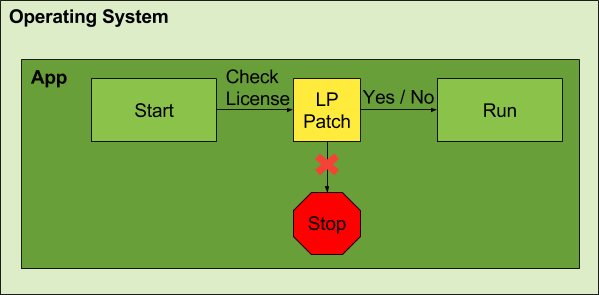
\includegraphics[width=0.8\textwidth]{data/verificationNowAttack.png}
    \caption{Attack on the license verification mechanism by \gls{luckypatcherg}}
    \label{fig:verificationNowAttack}
\end{figure}
